% concatenated from 3-Part2-InfiniteBhsets.tex
\documentclass[10pt,letterpaper]{article}

\usepackage{amsmath,amssymb,amsthm}
\usepackage{mathtools}
\usepackage{enumitem}
\usepackage[letterpaper,left=4cm,right=3cm,top=3cm,bottom=3cm]{geometry}
\usepackage{hyperref}
\usepackage{amsrefs}

\usepackage{tikz}
\usetikzlibrary{arrows.meta,decorations.pathreplacing,calc}
\usepackage{pgfplots}
\pgfplotsset{compat=1.18}

%--- draft-only: delete this block (and all \KO, \KOinline, \ko) at submission
\usepackage{todonotes}
\setlength{\marginparwidth}{3.5cm}
\newcommand{\KO}[1]{\todo[color=blue!10]{{\footnotesize K:} \footnotesize #1}}
\newcommand{\KOinline}[1]{\todo[inline,color=blue!10,author=Kevin]{#1}}
\newcommand{\ko}[1]{\textcolor{blue}{K: #1}}
%---

\newcommand{\NN}{\ensuremath{\mathbb N}}
\newcommand{\RR}{\ensuremath{\mathbb R}}
\newcommand{\cA}{\mathcal{A}}
\newcommand{\cB}{\mathcal{B}}
\newcommand{\cG}{\mathcal{G}}
\newcommand{\cS}{\mathcal{S}}

\DeclarePairedDelimiter{\abs}{\lvert}{\rvert}
\DeclarePairedDelimiter{\floor}{\lfloor}{\rfloor}
\DeclarePairedDelimiter{\ceiling}{\lceil}{\rceil}
\DeclarePairedDelimiter{\multi}{\{\!\{}{\}\!\}}
\newcommand{\multibinom}[2]{\left(\kern-0.3em\left(\genfrac{}{}{0pt}{}{#1}{#2}\right)\kern-0.3em\right)}
\DeclareMathOperator{\supp}{supp}
\DeclareMathOperator{\mult}{mult}

\newtheorem{thm}{Theorem}
\newtheorem{lem}[thm]{Lemma}
\newtheorem{cor}[thm]{Corollary}
\newtheorem{qst}[thm]{Question}
\newtheorem{cnj}[thm]{Conjecture}
\theoremstyle{remark}
\newtheorem{rem}[thm]{Remark}

\begin{document}
  \title{On the Thickness of Infinite Generalized Sidon Sets, II}
  \author{Kevin O'Bryant\thanks{Email: \texttt{kevin.obryant@csi.cuny.edu}.\\ 2020 Mathematics Subject Classification: 05B10, 11B83, 11B05.}}
  \date{\today}
  \maketitle

\begin{abstract}
A set $\cA$ of nonnegative integers is a $B_h$-set if the sums
$a_1+\cdots+a_h$ with $a_1\le\cdots\le a_h$ and $a_i\in\cA$ are distinct;
a $B_2$-set is a Sidon set. 
Write $A(n)=|\cA\cap[0,n)|$. We prove that for every even $h$ and every $B_h$-set $\cA$,
\[
  \liminf_{n\to\infty} \frac{A(n)}{\sqrt[h]{n/\log n}}
  \le \left(\frac{\pi}{\log 2} 
        \cdot \frac{\Gamma(1+h/2)^2}{\Gamma(1+1/h)^{h}}\right)^{1/h}.
\]
\end{abstract}

\section{Introduction}\label{sec:intro}
A set $\cA \subseteq \NN$ of nonnegative integers is a $B_h$-set if the sums 
  \[a_1+\cdots+a_h, \qquad a_1\le\cdots\le a_h, a_i\in\cA\] 
are distinct. 
A $B_2$-set is a Sidon set.
For a set $\cA\subseteq\NN$, we denote the counting function $|\cA\cap[0,n)|$ with the corresponding capital latin letter, e.g., $A(n)\coloneqq |\cA\cap[0,n)|$.  

\begin{thm}\label{thm:main}
Let $h$ be a positive even integer, and let $\cA$ be a $B_h$-set.
Then
  \[\liminf_{n\to\infty} \frac{A(n)}{\sqrt[h]{n/\log n}} \le 
  \left(\frac{\pi}{\log 2} \cdot \frac{\Gamma(1+\tfrac h2)^2}{\Gamma(1+\tfrac1h)^{h}}\right)^{1/h}.\]
\end{thm}

\begin{cor}%\limsup a_n / (n^h \log n)
  Let $\cA=\{0 \le a_1<a_2<\dots\}$ be an infinite $B_h$-set, $h$ even. Then
  \[\limsup_{n\to\infty} \frac{a_n}{n^h \log n} \ge \frac{\log 2}{\pi} \cdot \frac{h \, \Gamma(1+\tfrac1h)^{h}}{\Gamma(1+\tfrac h2)^2}\]
\end{cor}

Chen~\cite{1993.Chen} proved 35 years ago that this $\liminf$ is finite; our contribution is providing the explicit constant above, which we hope will spur further work. In Part I, the author proved a similar result for a different generalization of Sidon set, and in the case of $h=2$ Theorem~\ref{thm:main} reduces to a special case of that result. No result similar to Theorem~\ref{thm:main} is known for odd $h$, although Jia~\cite{1994.Jia} has conjectured one.

The best complementary result is Cilleruelo's construction~\cite{2014.Cilleruelo} of a $B_h$-set $\cG$ with
  \[G(n) = n^{\sqrt{(h-1)^2+1}-(h-1)+o(1)}.\]

\begin{figure}[t]% constant from Theorem~\ref{thm:main}
\centering
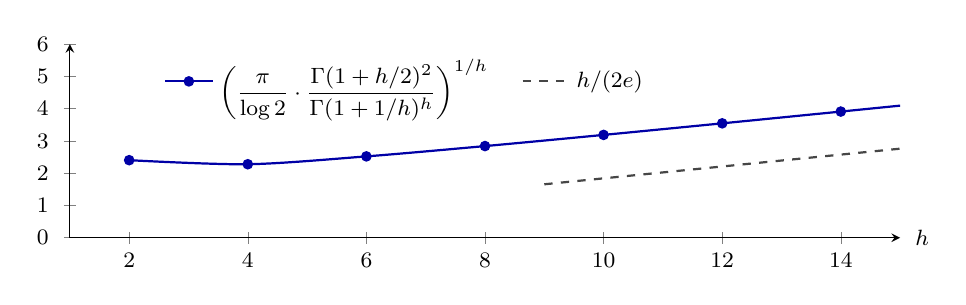
\begin{tikzpicture}
  \begin{axis}[
      width=\textwidth,
      height=0.3333\textwidth,
      xtick={2,4,6,8,10,12,14},
      xmin=1, xmax=15,
      ymin=0, ymax=6,
      ytick={0,1,2,3,4,5,6},
      axis lines=left,
      xlabel={$h$},
      xlabel style={at={(axis description cs:1,0)}, anchor=west, xshift=2pt},
      yticklabel style={xshift=-2pt},
      legend columns=-1,
      legend style={at={(0.5,0.98)}, anchor=north, xshift=-1cm, draw=none, fill=none, font=\footnotesize, /tikz/every even column/.append style={column sep=1em}},
      legend cell align=left,
      tick label style={font=\footnotesize},
      label style={font=\footnotesize},
    ]
    \addplot[
        color=blue!65!black, mark=*, mark size=1.5pt, thick, smooth,
      ] coordinates {
        (2, 2.4022)
        (4, 2.2765)
        (6, 2.5197)
        (8, 2.8390)
        (10, 3.1851)
        (12, 3.5434)
        (14, 3.9079)
      };
    \addlegendentry{$\left(\dfrac{\pi}{\log 2}\cdot\dfrac{\Gamma(1+h/2)^2}{\Gamma(1+1/h)^{h}}\right)^{1/h}$}

    % continuation of the blue curve past h=14, toward h=16, truncated at h=15 (no marker)
    \addplot[color=blue!65!black, thick, no marks, forget plot] coordinates {
        (14, 3.9079)
        (15, 4.0919)
      };

    \addplot[color=gray!55!black, dashed, thick, domain=9:15, samples=2]
      {x/(2*2.718281828459045)};
    \addlegendentry{$h/(2e)$}
  \end{axis}
\end{tikzpicture}
\caption{The constant of Theorem~\ref{thm:main}, together with its asymptote $h/(2e)$. Strangely, the minimum is at $h=4$.}
\label{fig:constant-vs-h}
\end{figure}

\subsection{History of the Problem}
Erd\H{o}s proved, and St\"ohr~\cite{1955.Stohr} recorded, that every infinite $B_2$-set satisfies
\begin{equation*}\label{eq:erdos}
   \liminf_{n\to\infty}\frac{A(n)}{\sqrt{n/\log n}} < C ,
\end{equation*}
with an unspecified absolute constant $C$; Erd\H{o}s's proof is given in~\cite{1966.Halberstam&Roth}.
In Part~I of this work~\cite{2026.Obryant-a}, the author proved the $h=2$ case of Theorem~\ref{thm:main}, and that if $\cG$ is a $g$-Golomb ruler (no $d$ arises more than $g$ times as a difference of elements of $\cG$, e.g., a Sidon set is a $1$-Golomb ruler), then
\begin{equation*}\label{eq:g-Golomb}
  \liminf_{n\to\infty}\frac{G(n)}{\sqrt{n/\log n}} \le 
  \sqrt{\frac{4g}{\log 2}}.
\end{equation*}

In a series of papers culminating in \cite{1993.Chen}, Nash~\cite{1989.Nash}, Jia~\citelist{\cite{1989.Jia} \cite{1994.Jia}}, Helm~\citelist{\cite{1993.Helm} \cite{1994.Helm}}, and finally Chen~\citelist{\cite{1993.Chen} \cite{1996.Chen}} showed that for every even integer $h$ and every $B_h$-set $\cA$,
  \[\liminf_{n\to\infty} \frac{A(n)}{\sqrt[h]{n/\log n}} < \infty.\]

\subsection{A brief description of our improvement}
Our own work follows Jia~\cite{1994.Jia}, with substantials detours for the sake of lowering the constant.

Following Erd\H{o}s, all previous authors had considered how a $B_h$-set intersects $[(\ell-1)N,\ell N)$, for $\ell\in \{1,\dots,N\}$, with $N\to \infty$. In~\cite{2026.Obryant-a}, the author found advantage in separating the width of the intervals and the number of intervals while studying $g$-Golomb rulers, and also averaged over shifts of the intervals. While the balance between number and width is different in this work, the idea originates in that work. Similarly, we reuse the weighted Cauchy's Inequality from that work. 

Lemma~\ref{lem:simplex} is new, giving a nontrivial lower bound on the size of a $k$-fold sumset of a $B_{2k}$-set $\cA$ under a lower bound hypothesis $A(n)$. 

All of the best work on $B_h$-sets proceeds by considering the differences of the $(h/2)$-fold sumset of $\cA$. 
This is why our result benefits from the hypothesis that $h$ is even, for example. 
Every $B_h$-set is also a $B_{h-1}$-set, so that our result extends to odd $h$, but only in that artifical manner. It is not known if
  \[\liminf_{n\to\infty} \frac{A(n)}{n^{1/h}} = 0 \]
for odd $h\ge 3$.

\section{Multiset notation and terminology}
In this work, a multiset $\beta$ is a function $\mult_\beta:\NN\to \NN$. 
We write $x\in \beta$ for $\mult_\beta(x) \ge 1$, and the cardinality and sum of a multiset is
\begin{align*}
  |\beta| & \coloneqq \sum_{x\in\NN} \mult_\beta(x) \\
  \Sigma \beta & \coloneqq \sum_{x\in \NN} \mult_\beta(x) \cdot x .
\end{align*}
The multiset $\emptyset$ has $\mult_\emptyset(x) = 0$ for all $x$.

The support of a multiset $\beta$ is the \emph{set} of integers with multiplicity at least $1$:
  \[\supp(\beta) \coloneqq \{ a : \mult_\beta(a)\ge 1\}.\]
We define the multiset intersection $\beta \Cap \delta$ and sum $\beta \uplus \delta$ through the $\mult$ function:
\begin{align*}
  x \in \beta &\qquad \Leftrightarrow\qquad \mult_\beta(x) \ge 1 \\
%  U = \beta \Cup \delta &\qquad \Leftrightarrow\qquad  \mult_U(x) = \max\{\mult_\beta(x),\mult_\delta(x)\} \\
  U = \beta \Cap \delta &\qquad  \Leftrightarrow\qquad  \mult_U(x) = \min\{\mult_\beta(x),\mult_\delta(x)\} \\
%  \beta \subseteq \delta &\qquad  \Leftrightarrow\qquad   \text{for all $x$: } \mult_\beta(x) \le \mult_\delta(x)\\
  U = \beta \uplus \delta &\qquad  \Leftrightarrow\qquad  \mult_U(x) = \mult_\beta(x)+\mult_\delta(x) 
%  U = \beta \setminus \delta &\qquad\Leftrightarrow\qquad  \mult_U(x) = \max\{\mult_\beta(x)-\mult_\delta(x),\,0\},
\end{align*}  
The usual set operations $\in, \cup, \cap$ apply to the supports of their arguments, e.g., $\beta \cap \delta \coloneqq \supp(\beta) \cap \supp(\delta)$ and $x\in \beta$ means $x\in \supp(\beta)$. We say that $\beta,\delta$ are \emph{disjoint} if $\beta\cap\delta = \emptyset$.

The set of all multisubsets with support contained in the set $X$ with cardinality $i$ is denoted $\multibinom{X}{i}$ (read ``$X$ multichoose $i$''), and by stars-and-bars we have the count
  \[\abs*{\multibinom{X}{i}}= \multibinom{\abs{X}}{i} = \binom{|X|+i-1}{i}.\]
We will use both sides of the standard bounds
  \[ \frac{|X|^i}{i!}\le \abs*{\multibinom{X}{i}} \le \frac{(|X|+i)^i}{i!}.\]

We write $\multi{a_1,\dots,a_i}$ for the multiset $\beta$ 

This next lemma is used frequently\footnote{Lemma~\ref{lem:cancel} has the same essence as the ubiquitous fact from elementary number theory: if $p,q$ are positive integers and $\gcd(p,q)=\gcd(p',q')=1$ and $pq'=p'q$, then $p=p'$ and $q=q'$.} to connect sumsets and difference sets of a $B_h$-set.
\begin{lem}\label{lem:cancel}
Let $P,P',Q,Q'$ be multisets with $P\cap Q=P'\cap Q'=\emptyset$.  If $P\uplus Q'=P'\uplus Q$, then $P=P'$ and $Q=Q'$.
\end{lem}

A quick example using multisets is enlightening, if ornate.
\begin{lem}\label{lem:B_h is B_p}
  Suppose that $\cA$ is a $B_h$-set and $1\le p \le h$. Then $\cA$ is a $B_p$-set. 
\end{lem}
\begin{proof}
If $\cA=\emptyset$ or $p=h$ or $p=1$, then the lemma is trivial , but true. 

Otherwise, suppose by way of contradiction that $a\in\cA$ and $\beta,\delta \in \multibinom{\cA}{p}$ with $\beta\neq \delta$ yet $\Sigma \beta = \Sigma \delta$. Let $\alpha$ be the multiset containing only $a$, and containing it with multiplicity $h-p$. Then
  \[\Sigma (\alpha \uplus \beta) = \Sigma(\alpha \uplus \delta),
  \qquad |\alpha \uplus \beta| = |\alpha \uplus \delta| =h.\]
By the $B_h$-property, $\alpha \uplus \beta = \alpha \uplus \delta$, contradicting $\beta \neq \delta$.
\end{proof}

If $\cA$ is a $B_h$-set, and $\beta,S \in \multibinom{\cA}{h}$ and $\Sigma \beta = \Sigma S$, then $\beta=S$. 
This is just a restatement of the $B_h$-property.
In other words, by the $B_h$-property (which implies the $B_p$ property for $1\le p\le h$), the elements of the $p$-fold sumset $p\cA$ are in bijective correspondence with $\multibinom{\cA}{p}$.

\begin{cor}\label{cor:Vs}
Let $\cA$ be a $B_h$-set and $1\le p\le h$. The map $\beta\mapsto\Sigma\beta$
is a bijection from $\multibinom{\cA}{p}$ onto the $p$-fold sumset $p\cA$.
\end{cor}

For $s\in p\cA$ we write $V_s$ for the unique preimage (specifying $p$ in context), so $\Sigma V_s=s$.

\section{Lemmata on $B_h$-sets}
We will use calligraphy letters for sets of nonnegative integers, a subscript for the truncation of the set, and the corresponding capital latin letter for the counting functions. To wit, for $\cS=k\cA$, the $k$-fold sumset of $\cA$, we have $\cS_W = \cS\cap[0,W)$ and
  \[S(W) = \abs*{\cS_W} = \abs*{\cS \cap [0,W)}.\]

Let $\cS = k\cA$, with counting function $S(n)$. A $B_2$-set not only has distinct sums, it also has distinct differences. While the set $\cS$ is \emph{not} a $B_2$-set, we are able to control its differences, and that control drives our bound on the ``energy'' of $\cS$ relative to a partition of $\NN$.

Our first result connects an ``energy'' quantity (sum of squares) to the $\liminf$. 

\begin{lem}\label{lem:energy}
Let $\cB\subseteq\NN$ have counting function $B(n)$.
Let $M=M(N)$ satisfy, as $N\to\infty$,
\begin{enumerate}[label=\textit{(\roman*)},noitemsep]
  \item\label{eng:window} $B((M+1)N)=o(N)$;
  \item\label{eng:ratio} $\log M/\log N =1+o( 1 )$;
  \item\label{eng:head} $B(N)=o(\sqrt{N \log N})$.
\end{enumerate}
Suppose there is a constant $c$ such that there is an
offset $t^\ast=t^\ast(N)\in[0,N)$ whose block counts
  \begin{equation*}\label{hyp:blocks}
    F_\ell \coloneqq B(t^\ast+\ell N)- B(t^\ast+(\ell-1)N)
  \end{equation*}
satisfy (as $N\to\infty$)
  \begin{equation}\label{hyp:energy}
    \sum_{\ell=1}^{M}\binom{F_\ell}{2}\le cN+o(N).
  \end{equation}
Then
  \[\liminf_{m\to\infty}\frac{B(m)}{\sqrt{m/\log m}}\le \sqrt{\frac{8c}{\log 2}}.\]
\end{lem}

We begin with the simple bound on the size of a $B_h$-set in $[0,m)$. We remark that there is a large literature around improving the constant in Lemma~\ref{lem:easy Bh bound}. For $h>2$, the correct constant is unknown, and for $h=2$ the correct error term is unknown. For the purposes of this work, surprisingly, Lemma~\ref{lem:easy Bh bound} suffices.

\begin{lem}\label{lem:easy Bh bound}
  If $\cG$ is a $B_h$-set and $m\ge 1$, then $G(m) \le (h\cdot h!)^{1/h} \cdot m^{1/h}$.
\end{lem}

\begin{proof}
  There are $G(m)^h$ tuples of numbers (each with $h$ entries) in $\cG_m$, each tuple has sum in $[0,mh)$, and by the $B_h$-property each number in $[0,mh)$ can be the sum of at most $h!$ different tuples. Thus,
  \(\frac{G(m)^h}{h!} \le mh.\)
\end{proof}

In particular,
  \[ A(n) = O(n^{1/h}).\]
We also have some immediate bounds from the multiset characterization of the $B_h$-property in Corollary~\ref{cor:Vs}. For example, we have $k\cA_n \subseteq[0,kn)$, so that
  \begin{equation}\label{eq:S(kn) > A(n)^k / k!}
    S(kn) \ge \abs*{\multibinom{\cA_n}{k}} = \binom{A(n)+k-1}{k} \ge \frac{A(n)^k}{k!}.
  \end{equation}
We work harder to produce a better bound in Lemma~\ref{lem:simplex} below.
\begin{lem}[Lower bound on $S(m)$]\label{lem:simplex}
Let $h=2k$ be even, let $\cA$ be a $B_h$-set, and suppose there are $\tau>0$
and $n_0\ge e$ such that
  \[A(x) \ge \tau\left(\frac{x}{\log x}\right)^{1/h}
    \qquad\text{for all } x> n_0.\]
Then $\cS=k\cA$ satisfies,
  \[\liminf_{m\to\infty} \frac{S(m)}{\sqrt{m/\log m}} \ge \frac{2\tau^k \Gamma(1+\tfrac1h)^k}{k!\sqrt{\pi}}.\]
\end{lem}
 
\begin{proof}
Set $f(x) \coloneqq \tau(x/\log x)^{1/h}$. Since
  \[\frac{f'(x)}{f(x)} = \frac{1}{hx}\left(1-\frac{1}{\log x}\right),\]
$f$ is continuous, strictly increasing, and unbounded on $[e,\infty)$; we assume that $n_0\ge e$. 
In particular $A(x)\ge f(x)$ for $x> n_0$, so $\cA$ is infinite; write 
  \[\cA = \{0\le a_1 < a_2<\cdots\}.\]
For integers $j\ge J_0\coloneqq \floor{f(n_0)}+1$, let $x_j$ be the unique solution to $f(x_j)=j$. The schematic in Figure~\ref{fig:x and y} illustrates these relationships.

\begin{figure}[t]
\begin{center}
\resizebox{\textwidth}{!}{%
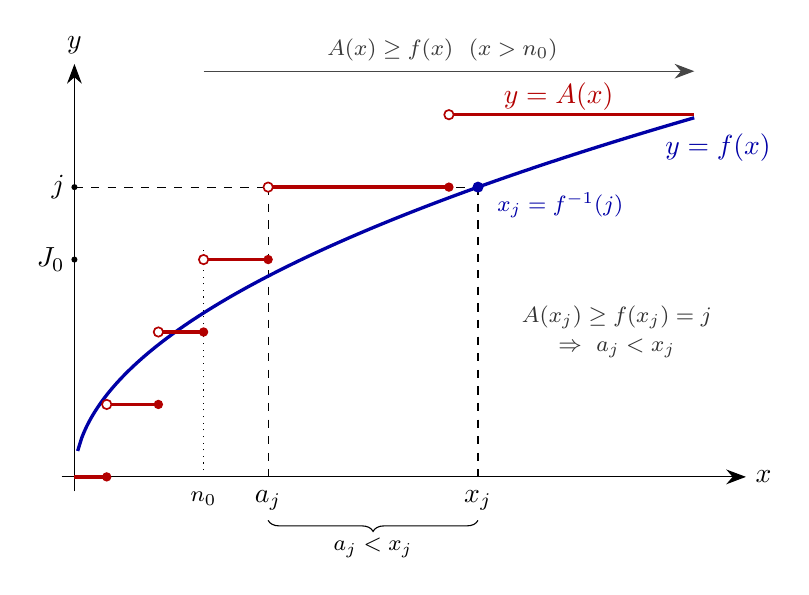
\begin{tikzpicture}[>={Stealth[length=2.5mm]}, x=0.82cm, y=0.92cm]

  %% dot styles for the jumps
  \tikzset{
    closed/.style={red!70!black, fill=red!70!black},
    open/.style  ={red!70!black, fill=white, line width=0.6pt}}

  %% ---- axes ----
  \draw[->] (-0.2,0) -- (10.4,0) node[right] {$x$};
  \draw[->] (0,-0.2) -- (0,5.7) node[above] {$y$};

  %% ================= focus level  y = j  (drawn first, sits behind) ==========
  \def\aj{3.0}    % a_j : where the staircase first reaches height j
  \def\xj{6.25}   % x_j : where the curve reaches height j,  f(x_j)=j
  \def\jj{4}      % the integer level j

  \draw[dashed] (0,\jj) -- (\xj,\jj);
  \draw[dashed] (\aj,\jj) -- (\aj,0);
  \draw[dashed] (\xj,\jj) -- (\xj,0);
  \node[left] at (0,\jj) {$j$};
  \fill (0,\jj) circle (1.1pt);

  %% starting index J_0 = floor(f(n_0))+1 on the y-axis
  \node[left] at (0,3) {$J_0$};
  \fill (0,3) circle (1.1pt);

  %% ---- threshold n_0 ----
  \draw[dotted] (2.0,0) -- (2.0,3.2);
  \node[below, font=\footnotesize] at (2.0,-0.08) {$n_0$};

  %% ---- smooth lower bound f(x)=tau (x/log x)^{1/h}  (schematic: 1.6*sqrt x) ----
  \draw[very thick, blue!65!black, domain=0.05:9.6, samples=140, smooth]
        plot (\x, {1.6*sqrt(\x)});
  \node[blue!65!black, anchor=west] at (9.0,4.55) {$y=f(x)$};

  %% ---- A(x)=|A cap [0,x)| : horizontal treads only (no risers) ----
  %%  left-continuous:  closed dot on the right end, open dot on the left end.
  %%  x<n_0 : below the curve (no bound);  x>=n_0 : A(x) >= f(x), above the curve.
  \def\tread#1#2#3{% #1=x_left  #2=x_right  #3=height
    \draw[very thick, red!70!black] (#1,#3) -- (#2,#3);
    \draw[open]   (#1,#3) circle (1.7pt);
    \fill[closed] (#2,#3) circle (1.7pt);}
  \draw[very thick, red!70!black] (0,0) -- (0.5,0);
  \fill[closed] (0.5,0) circle (1.7pt);
  \tread{0.5}{1.3}{1}   % below n_0
  \tread{1.3}{2.0}{2}   % below n_0
  \tread{2.0}{3.0}{3}   % above (x>=n_0)
  \tread{3.0}{5.8}{4}   % above  -- this is the level-j tread
  \draw[very thick, red!70!black] (5.8,5) -- (9.6,5);
  \draw[open] (5.8,5) circle (1.7pt);
  \node[red!70!black, anchor=west] at (6.5,5.25) {$y=A(x)$};

  %% region where the hypothesis holds
  \draw[->, gray!55!black] (2.0,5.6) -- (9.6,5.6);
  \node[gray!45!black, font=\footnotesize, anchor=south] at (5.7,5.6)
        {$A(x)\ge f(x)\ \ (x> n_0)$};

  %% marked intersection at height j on the curve (the open dot at (a_j,j)
  %% already comes from the level-j tread: A(a_j)=j-1, value attained for x>a_j)
  \fill[blue!65!black] (\xj,\jj) circle (2pt);  % curve reaches j at x_j
  \node[blue!65!black, anchor=west, font=\footnotesize]
        at (\xj+0.15,\jj-0.25) {$x_j=f^{-1}(j)$};

  %% x-axis labels and the resulting inequality
  \node[below] at (\aj,-0.05) {$a_j$};
  \node[below] at (\xj,-0.05) {$x_j$};
  \draw[decorate,decoration={brace,amplitude=4pt,mirror}]
        (\aj,-0.6) -- (\xj,-0.6)
        node[midway,below=3pt,font=\footnotesize] {$a_j<x_j$};

  %% the mechanism
  \node[align=center, font=\footnotesize, gray!40!black]
        at (8.4,2.0)
        {$A(x_j)\ge f(x_j)=j$\\[1pt]$\Rightarrow\ a_j<x_j$};
  \end{tikzpicture}}
\end{center}
\caption{Schematic showing the relationships $A(x)\ge f(x)$ for $x> n_0$, $f(x_j)=j$, and $a_j < x_j$.}
\label{fig:x and y}
\end{figure}

Moreover, since $A(x_j) \ge f(x_j)=j$ for $j\ge J_0$, we see that \(a_j < x_j \qquad (j\ge J_0).\)
Suppose $J_0\le j_1\le\cdots\le j_k$ are integers with $x_{j_1}+\cdots+x_{j_k}\le m$. The multiset $\beta\coloneqq \multi{a_{j_1},\dots,a_{j_k}}\in\multibinom{\cA}{k}$ has $\Sigma\beta=\sum a_{j_i}< \sum x_{j_i} <m$. Also, distinct $\beta$ produce distinct elements of $\cS\cap[0,m)$ by Corollary~\ref{cor:Vs}. 
Hence
  \begin{align*}
    S(m) 
    &\ge \#\left\{(j_1,\dots,j_k) : J_0\le j_1\le\cdots\le j_k,
        \sum_{i=1}^k x_{j_i}\le m\right\} \\
    &\ge \frac{1}{k!} \#\left\{(j_1,\dots,j_k)\in\{J_0,J_0+1,\dots\}^k :
    \sum_{i=1}^k x_{j_i}\le m\right\} \\
    &=: \frac{1}{k!} N^*(m).
  \end{align*}
We have successfully transformed bounding $S(m)$, a number theory problem, with counting the lattice points in a region of $\RR^k$. Unsurprisingly, we proceed by replacing the lattice point count with an integral, a Dirichlet integral, and will arrive at (for $m\ge \exp(f^{-1}(J_0)+1)$)
  \begin{equation*}
    N^{*}(m) \ge \frac{\tau^k}{h^k(\log m)^{1/2}} \left( 1-\frac{1}{\log \log m} \right)^k
  \left(\frac{2\Gamma(\tfrac1h)^k}{\sqrt{\pi}}\sqrt m - k h^k \left(\frac{\log m}{m}\right)^{1/h}\sqrt{m}\right),
  \end{equation*}
from which Lemma~\ref{lem:simplex} follows by routine asymptotic analysis.

Each integer tuple $(j_1,\dots,j_k)$ corresponds to the unit box $\prod_{i}(j_i-1,j_i]$, and on that box $\lceil y_i\rceil=j_i$. 
Therefore
  \[N^{*}(m) = \operatorname{vol}\left\{(y_1,\dots,y_k) \in (J_0-1,\infty)^k :
     \sum_{i=1}^k x_{\lceil y_i\rceil}\le m\right\}.\]
The function $f$ has an inverse on $[e,\infty)$ that is also continuous and strictly increasing. 
For $\ceiling{y_i}\ge J_0$, we have $f^{-1}(y_i+1)\ge f^{-1}(\ceiling{y_i}) = x_{\ceiling{y_i}}$.
Hence
  \begin{multline*}
    \left\{ (y_1,\dots,y_k) \in (J_0-1,\infty)^k : y_i > J_0,
     \sum_{i=1}^k f^{-1}(y_i+1) \le m\right\}\\
     \subseteq
     \left\{(y_1,\dots,y_k) \in (J_0-1,\infty)^k :
     \sum_{i=1}^k x_{\lceil y_i\rceil}\le m\right\}.
  \end{multline*}
The substitution $u_i\coloneqq f^{-1}(y_i+1)$, with $dy_i=f'(u_i)du_i$ and
$u_0\coloneqq \max\{\log m, f^{-1}(J_0+1)\}$, gives
  \[N^{*}(m) \ge \int_{\substack{u_i>u_0\\ u_1+\cdots+u_k\le m}}
     \prod_{i=1}^k f'(u_i)\,du_i.\]
 

By calculus, we have for $u>u_0$
  \begin{align*}
    f'(u) 
    &= \frac{\tau}{h} \frac{u^{1/h-1}}{(\log u)^{1/h}} \left( 1-\frac{1}{\log u} \right) \\
    &\ge \frac{\tau}{h(\log m)^{1/h}} \left( 1-\frac{1}{\log u_0} \right) u^{1/h-1},
  \end{align*}
and $f'>0$.
Thus,
  \[N^{*}(m) \ge \frac{\tau^k}{h^k(\log m)^{k/h}} \left( 1-\frac{1}{\log u_0} \right)^k
  \int_{\substack{u_i>u_0\\ u_1+\cdots+u_k\le m}}
     \prod_{i=1}^k u_i^{1/h-1} \,du_i.\]

Dirichlet's integral technique~\cite{1927.Whittaker&Watson}*{page 258--9} evaluates the untruncated version:
  \[\int_{\substack{u_i>0\\ u_1+\cdots+u_k\le m}}
     \prod_{i=1}^k u_i^{1/h-1}\,du_i
     %= \frac{\Gamma(\tfrac1h)^k}{\Gamma(1+\tfrac kh)}m^{k/h}
     = \frac{2\Gamma(\tfrac1h)^k}{\sqrt{\pi}}\sqrt m.\]
The truncation costs little: the portion of the untruncated integral with $u_1\le u_0$ is at most
  \[\int_0^{u_0}u^{1/h-1}\,du\cdot
    \left(\int_0^m u^{1/h-1}\,du\right)^{k-1}
    = h^k u_0^{1/h} m^{(k-1)/h} = o(\sqrt{m}),\]
and by symmetry the total cost is at most $k$ times this. 
We now have
  \begin{align*}
    N^{*}(m) 
    &\ge \frac{\tau^k}{h^k(\log m)^{1/2}} \left( 1-\frac{1}{\log u_0} \right)^k
  \left(\frac{2\Gamma(\tfrac1h)^k}{\sqrt{\pi}}\sqrt m - o(\sqrt m)\right)\\
    &\le \frac{2\tau^k \Gamma(\tfrac1h)^k}{\sqrt{\pi} h^k} \frac{\sqrt{m}}{\sqrt{\log m}} \left( 1-\frac{k}{\log \log m} \right)
  \left(1 - o(1)\right)\\
  &= (1-o(1)) \frac{2\tau^k \Gamma(1+\tfrac1h)^k}{\sqrt{\pi}} \frac{\sqrt{m}}{\sqrt{\log m}}.
  \end{align*}
This is the bound reported in Lemma~\ref{lem:simplex}.
\end{proof}

We also have $\cS_n \subseteq k\cA_n$, so that
  \begin{multline}\label{eq:S(n) = O(sqrt n)}
    S(n) \le |k\cA_n| = \abs*{\multibinom{\cA_n}{k}} \\
  \le (A(n)+k-1)^k = (O(n^{1/h})+k-1)^k = O(n^{k/h})=O(n^{1/2}).
  \end{multline}

We begin now with the critical task: controlling the differences of $\cS$ to produce the upper bound on $\sum \binom{F_\ell}{2}$ required by Lemma~\ref{lem:energy}.

For nonnegative integers $r,p,q,x,L$, let
\begin{align*}
  T(p,q;x,L)
  &\coloneqq \{(\beta,\delta)\in \multibinom{\cA}{p} \times \multibinom{\cA}{q} :
     \beta\cap\delta=\emptyset,x<\Sigma\beta-\Sigma\delta<L+x\} \\
  \Phi(r,p,q;x,L)
   &\coloneqq \left\{(\vec a;\beta,\delta):
     \vec a \in (\cA_L)^r , 
     (\beta,\delta) \in T(p,q;x,L)\right\}.
\end{align*}
Note that $\beta,\delta$ are multisets taken from $\cA$, not from $\cA_L$, but $\vec a = (a_1,\dots,a_r )$ is an ordered tuple of elements from $\cA_L$, possibly with repetitions. This asymmetry is useful because the
$a_i$ range freely over $\cA_L$ and that allows us to factor nicely:
\begin{equation}\label{eq:factor Phi}
   \abs*{\Phi(r ,p,q;x,L)} = \abs*{\cA_L}^r \abs*{T(p,q;x,L)}.
\end{equation}
In this work, we will use $x=0$ only. In Part III of this series, we will use the following lemma with $x$ varying.

We write $\Sigma \vec a$ for the sum of the entries of the tuple $\vec a$.

An important insight of Jia~\cite{1994.Jia} is that one needs to bound $\abs{\Phi}$, not $|T|$ alone.
Jia gives the following lemma with the conclusion $\abs{\Phi} = O(L)$. 
We have made it quantitative to ease our concerns over which constants depend on which, and the circular reasoning such confusion can enable. 
Certainly, the specific form of $C(r,p,q)$ is not germane to our usage.

\begin{lem}[Jia]\label{lem:jia}
Let $\cA$ be a $B_{h}$-set (with $h$ not necessarily even) and let $r,p,q\ge0$ satisfy $r+p+q\le h$.  
Then for every $x \ge 0$ and $L \ge 1$,
\[
   \abs*{\Phi(r,p,q;x,L)} \le L \cdot C(r,p,q),
\]
where \(c_0 \coloneqq (r+1)\frac{(r+p)!}{p!}\) and \(C(r,p,q) \coloneqq c_0 \sum_{j=0}^{q}(2r)^{j}.\)
\end{lem}

\begin{proof}
We induct on $q$, using $q=0$ as our base case.

With $q=0$, any $(\beta,\delta)\in T(p,0;x,L)$ has $\delta=\emptyset$ and $x<\Sigma\beta<L+x$. Consider the map taking 
$(\vec a;\beta)$ to $m\coloneqq \Sigma \vec a + \Sigma\beta$.  We have $x < m < (r+1)L+x$, giving $(r+1)L$ possibilities for $m$.  If two tuples share
$m$, then $\multi{a_1,\dots,a_r } \uplus \beta$ and $\multi{a_1',\dots,a_r'}\uplus\beta'$ are size $(r+p)$ multisets with the same sum $m$. As $r+p\le h$ and $\cA$ is a $B_h$-set,
  \[\multi{a_1,\dots,a_r}\uplus\beta = \multi{a_1',\dots,a_r'}\uplus\beta';\]
call this multiset $G$. 
The elements of the multiset $G$ can be listed in at most $(r+p)!$ ways, and the ordering of the entries that will be put into $\beta$ is irrelevant, so there are at most $(r+p)!/p!$ tuples $(\vec a;\beta) \in \cA^r \times \multibinom{\cA}{p}$.  Hence 
  \[\abs*{\Phi(r ,p,0;x,L)} \le \frac{(r +p)!}{p!} (r+1)L=c_0L = L \cdot C(r,p,0),\]
which establishes the base of our induction.

We now assume that $q\ge 1$, that for every $x\ge 0$ and $L\ge 1$ we have
  \[\abs{\Phi(r,p,q-1;x,L)} \le L\cdot C(r,p,q-1),\] 
and that $r+p+q \le h$, and will show that 
  \[\abs*{\Phi(r,p,q;x,L)} \le L\cdot C(r,p,q) = c_0L + r \cdot 2L\cdot c_0 \sum_{j=0}^{q-1}(2r )^j.\]

We split the count into two cases: $((a_1,\dots,a_r );\beta,\delta)\in \Phi(r,p,q;x,L)$ where no $a_i$ is in $\delta$, and where some $a_i \in\delta$ and we can use the induction hypothesis.

First, we suppose that no $a_i$ is in $\delta$. Map
$(\vec a;\beta,\delta)\in \Phi(r,p,q;x,L)$ to $\Sigma\vec a+\Sigma\beta - \Sigma\delta =: m$,
so $x< m<(r+1)L+x$ and there are fewer than $(r+1)L$ choices for $m$.  If two tuples map to the same $m$, then we have two multisets with $r+p+q$ elements in a $B_{r+p+q}$-set (since $r+p+q \le h$) having the same sum, and so the multisets are equal:
  \[\multi{a_1,\dots,a_r } \uplus \beta \uplus \delta'=\multi{a_1',\dots,a_r '} \uplus \beta'\uplus\delta\] 
Put $P=\multi{a_1,\dots,a_r } \uplus \beta$, $Q=\delta$, $P'=\multi{a_1',\dots,a_r '}\uplus\beta'$, $Q'=\delta'$ into Lemma~\ref{lem:cancel}, and we conclude that $P=P'$ and $\delta=\delta'$. Thus each value of $m$ determines $\delta$ and the unique multiset $\multi{a_1,\dots,a_r } \uplus \beta$, and the latter splits into $(\vec a;\beta)$ in at most $(r +p)!/p!$ ways. Thus, there are at most $\frac{(r +p)!}{p!}(r +1)L=c_0L$ tuples $(\vec a;\beta,\delta)$ with no $a_i$ in $\delta$.

The case where some $a_i\in\delta$ is a touch more involved. To start, we can make a count with the assumption that $a_1\in \delta$, and then multiply by $r$ to get an upper bound on the number of tuples with \emph{some} $a_i\in\delta$. Delete one copy of $a_1$ from $\delta$ to get $\delta^- \in \multibinom{\cA}{q-1}$ and $\multi{a_1}\uplus \delta^- = \delta$. We have $\beta \cap \delta^-=\emptyset$ and
  \[x < \Sigma\beta-\Sigma\delta^- = (\Sigma\beta-\Sigma\delta)+a_1 < 2L+x,\] 
so $(\vec a; \beta, \delta^-) \in \Phi(r ,p,q-1;x,2L)$. 
By the induction hypothesis,
  \[\abs*{\Phi(r ,p,q-1;x,2L)} \le 2L \cdot C(r,p,q-1)
  = 2L \cdot c_0\sum_{j=0}^{q-1} (2r )^j.\]
Putting the first element of $\vec a$ back into $\delta$ does not increase the count, which stands at: at most
  \[ r  \cdot 2L \cdot c_0 \sum_{j=0}^{q-1} (2r )^j.\]

The two cases combine to give at most
  \[\abs*{\Phi(r ,p,q;x,L)} \le c_0L + r \cdot 2L \cdot c_0\sum_{j=0}^{q-1} (2r )^j 
    = L \cdot c_0 \sum_{j=0}^{q} (2r )^j,\]
as needed to complete the induction.
\end{proof}

The particular instance we will use follows.
\begin{lem}\label{lem:Jia in action}
For all $N\ge 1$ and $1\le r <k$, one has
  \[\abs*{\Phi(2r,k-r,k-r;0,N)} \le N \cdot C(2r,k-r,k-r).\]
  %(2r +1) \frac{(k+r)!}{(k-r)!} \sum_{j=0}^{k-r}(4r)^{j}.\]
\end{lem}

\begin{lem}\label{lem:sumset energy bound}
Let $h$ be even, let $\cA$ be a $B_h$-set satisfying 
  \begin{equation}\label{eq:tau appears}
    A(n) \ge \tau \, \left(\frac{n}{\log n}\right)^{1/h}
  \end{equation}
for some $\tau\ge 0$ and all $n\ge n_0\ge 3$. let $k \coloneqq h/2$, and let $\cS=k\cA$. For each $N\ge n_0$, there is a $t^\ast\in [0,N)$ that makes the block counts 
  \[F_\ell\coloneqq S(t^\ast+\ell N) - S(t^\ast+(\ell-1)N)\]
    %\abs*{\cS\cap[t^\ast+(\ell-1)N, t^\ast+\ell N)}\] 
satisfy, with $M\coloneqq \floor{N/\log^3(N)}$,
  \[   \sum_{\ell=1}^{M}\binom{F_\ell}{2} \le \frac{1}{2}\,N + o(N).\]
\end{lem}

\begin{proof}
For $N\ge 3$, put $W\coloneqq (M+1)N=N^2/\log^3(N)+O(N)$.  For integers
$t\in[0,N)$ and $\ell \in [1,M]$, set
  \[F_\ell^{(t)}\coloneqq \abs*{\cS \cap [t+(\ell-1)N, t+\ell N)}
  =S(t+\ell N)-S(t+(\ell-1)N).\]  
A pair $(s,s') \in \cS_W\times \cS_W$ with $s-s'=d \in[1, N)$, lies in a common block $[t+(\ell-1)N, t+\ell N)$ for at most $N-d$ offsets, so
\begin{equation}\label{eq:average}
   \frac1N\sum_{t=0}^{N-1}\sum_{\ell=1}^{M}\binom{F_\ell^{(t)}}{2}
    \le \frac1N\sum_{d=1}^{N-1}(N-d) P(d),
\end{equation}
where $P(d)$ is the number of such pairs with difference $d$.  
That is,
  \[P(d) \coloneqq \#\left\{ (s,s') \in (\cS_W)^2 \colon s-s'=d \right\}.\]
Choose $t^\ast\in[0,N)$ so that
  \[\sum_{\ell=1}^{M}\binom{F_\ell^{(t^\ast)}}{2} \le \frac1N\sum_{t=0}^{N-1}\sum_{\ell=1}^{M}\binom{F_\ell^{(t)}}{2}\]
and set $F_\ell \coloneqq F_\ell^{(t^\ast)}$. We have
  \begin{equation}\label{eq:P appears}
    \sum_{\ell=1}^{M}\binom{F_\ell}{2}
    \le \frac1N\sum_{d=1}^{N-1}(N-d) P(d).
  \end{equation}

For each $s\in \cS$, we identify the unique $V_s \in \multibinom{\cA}{k}$ with $\Sigma V_s =s $ (unique because $\cA$ is a $B_k$-set by Lemma~\ref{lem:B_h is B_p}). 
We stratify $P(d)$ by the size of $V_s \Cap V_{s'}$. Namely, set
  \[P_r(d) \coloneqq \#\left\{ (s,s')\in (\cS_W)^2 \colon s-s'=d ,\abs*{V_s \Cap V_{s'}}=r \right\}.\]
We have, $P(d) = \sum_{r=0}^k P_r(d)$. For $d\ge1$, we have $P_k(d)=0$, as $|V_s \Cap V_{s'}| =k$ implies that $V_s=V_{s'}$, so that $s=s'$ and $s-s'=d=0$. 
Thus, Line~\eqref{eq:P appears} becomes
  \begin{equation}\label{eq:P_r appears}
    \sum_{\ell=1}^{M-1}\binom{F_\ell}{2}
    \le \frac1N\sum_{d=1}^{N-1}(N-d) P_0(d)+ \sum_{r=1}^{k-1} \frac1N\sum_{d=1}^{N-1}(N-d) P_r(d).
  \end{equation}

We now show that for $d\ge 1$, we have $P_0(d)\le 1$. 
We see that $P_0(d)$ counts the number of pairs $(s,s')\in (\cS_W)^2$ with $s-s'=d$ and $V_s \Cap V_{s'}=\emptyset$.
Suppose that both $(s,s')$ and $(u,u')$ are such pairs. 
Then $s+u'=u+s'$, an identity of $2k$-fold sums, so by the $B_{2k}$ property
  \[V_s \uplus V_{u'} = V_{u} \uplus V_{s'}.\]
By Lemma~\ref{lem:cancel}, $V_s=V_u$ and $V_{s'}=V_{u'}$, from which it follows that $s=u$ and $s'=u'$. 

Therefore
\begin{equation}\label{eq:disjoint}
   \frac1N \sum_{d=1}^{N-1}(N-d) P_0(d) \le \frac 1N \sum_{d=1}^{N-1}(N-d) = \frac12 (N-1).
\end{equation}
The bound~\eqref{eq:P_r appears}, with $N-d \le N$ becomes
  \begin{equation}\label{eq:P_0 is gone}
    \sum_{\ell=1}^{M-1}\binom{F_\ell}{2}
    \le \frac12 N + \sum_{r=1}^{k-1} \sum_{d=1}^{N-1} P_r(d).
  \end{equation}

We now consider $1 \le r < k$, and show that for each such $r$ we have $\sum_d P_r(d)=o(N)$.  
Consider a pair $(s,s')$ counted by $\sum_{d=1}^{N-1} P_r(d)$, so that there are unique $\alpha\in \multibinom{\cA}{r}, \beta,\delta \in \multibinom{\cA}{k-r}$ with $\alpha =V_s \Cap V_{s'}$ (so $\abs{\alpha}=r$), $V_s = \alpha \uplus \beta$ and $V_{s'} = \alpha \uplus \delta$ (so $\abs{\beta}=k-r = \abs{\delta}$). 
Note that $\beta \cap \delta = \emptyset$, since at each $x$ either $\mult_\beta(x)=0$ or $\mult_\delta(x)=0$.
The map from $(s,s')$ to $(\alpha;\beta,\delta)$ is injective. 
Since $\Sigma \beta -\Sigma\delta =s-s' =d \in [1,N)$, we see that $(\beta,\delta) \in T(k-r,k-r;0,N)$.

Hence, using $r\ge 1$ we have the bound $\binom{A(W)+r-1}{r}\le A(W)^{r}$, and so
\[
   \sum_{d=1}^{N-1}P_r(d)
   \le \abs*{\multibinom{\cA_W}{r}}\cdot\abs*{T(k-r,k-r;0,N)}
   \le A(W)^{r} \abs*{T(k-r,k-r;0,N)}.
\]
Now multiply and divide by $A(N)^{2r}$ and apply the factorization~\eqref{eq:factor Phi} to get
\begin{align*}
   \sum_{d=1}^{N-1}P_r(d)
   &\le\frac{A(W)^{r}}{A(N)^{2r}}\cdot A(N)^{2r} \abs*{T(k-r,k-r;0,N)}\\
   &=\frac{A(W)^{r}}{A(N)^{2r}} \abs*{\Phi(2r,k-r,k-r;0,N)}.
\end{align*}
Lemma~\ref{lem:Jia in action} gave us
\[
   \abs*{\Phi(2r,k-r,k-r;0,N)}\le N \cdot C(2r,k-r,k-r),
\]
bringing our bound to
  \[\sum_{d=1}^{N-1} P_r(d) \le  C(2r,k-r,k-r) \, \frac{A(W)^{r}}{A(N)^{2r}}\,  N.\]


It remains to see that $A(W)^r/A(N)^{2r}=o(1)$. This is why Jia introduced a growth regularity hypothesis $A(N^2) = O(A(N)^2)$. As Erd\H{o}s, Helm, and Jia weren't thinking of producing explicit constants, they never separated $M$ to be its own parameter, and just used $M=N$. The flexibility afforded by this additional parameter is what allows our argument to proceed without Jia's regularity hypothesis. That is, this step is why we have $M=N/\log^3 N$ and not $M=N/\log N$ (as in Part I of this series of papers) or $M=N$ (as in Chen's work).

By Lemma~\ref{lem:easy Bh bound} and
$W=N^2/\log^3 N$,
\[
   A(W)\le(h\cdot h!)^{1/h}W^{1/h}
   =(h\cdot h!)^{1/h} \frac{N^{2/h}}{\log^{3/h} N},
\]
while~\eqref{eq:tau appears} gives $A(N)\ge \tau N^{1/h}/\log^{1/h} N$ for
$N\ge n_0$.  Therefore
\[
   \frac{A(W)^{r}}{A(N)^{2r}}
   \le\frac{(h\cdot h!)^{r/h}}{\tau^{2r}} 
     \frac{\log^{-3r/h} N}{\log^{-2r/h} N}
   =\left(\frac{(h\cdot h!)^{1/h} / \tau^{2}}{\log^{1/h} N}\right)^r,
\]
which goes to $0$ as $N\to \infty$.
Combining, for each fixed $1\le r\le k-1$,
  \[
   \sum_{d=1}^{N-1}P_r(d)
   \le\frac{(h\cdot h!)^{r/h} C(2r,k-r,k-r)}{\tau^{2r}}\cdot
     \frac{N}{\log^{r/h} N}=O\left(\frac{N}{\log^{1/h} N}\right),
  \]
so the finite sum $\sum_{r=1}^{k-1}\sum_{d}P_r(d)=o(N)$.  The bound on Line~\eqref{eq:P_0 is gone} becomes
  \[   \sum_{\ell=1}^{M-1}\binom{F_\ell}{2}\le\frac{N}{2}+o(N), \]
which concludes the proof of Lemma~\ref{lem:sumset energy bound}.
\end{proof}


 

\section{The proof of Theorem~\ref{thm:main}}\label{sec:main proof} 
We now assemble the lemmas of the previous section into a proof of Theorem~\ref{thm:main}.

\begin{proof}
Assume, by way of contradiction, that
  \begin{equation}\label{eq:contradiction hypothesis}
    A(x) \ge \tau \left(\frac{x}{\log x}\right)^{1/h}
    \qquad \text{and} \qquad
    \tau >
    \left(\frac{\pi}{\log 2} \cdot \frac{\Gamma(1+\tfrac h2)^2}{\Gamma(1+\tfrac1h)^{h}}\right)^{1/h}
  \end{equation}
for all $x\ge n_0\ge 3$.

Let $k=h/2$, and let $\cS=k\cA$ be the $k$-fold sumset with counting function $S(n)\coloneqq \abs{\cS\cap[0,n)}$. By \eqref{eq:S(n) = O(sqrt n)} we have $S(n)=O(n^{1/2})$. With $M=\floor{N/\log^3 N}$, we have (as $N\to \infty$)
\begin{enumerate}[label=\textit{(\roman*)},noitemsep]
  \item $S((M+1)N)= O(((M+1)N)^{1/2}) = O(\frac{N}{\log^{3/2} N}) = o(N)$;
  \item $\log(M)/\log(N) \to 1$;
  \item $S(N) = O(N^{1/2}) = o(\sqrt{N\log N})$.
\end{enumerate}
By Lemma~\ref{lem:sumset energy bound}, there is a $t^\ast\in[0,N)$ with
  \[\sum_{\ell=1}^M \binom{F_\ell}{2} \le \frac12 N + o(N).\]
We satisfy the hypotheses of Lemma~\ref{lem:energy} with $c=1/2$, and so we conclude that
  \[\liminf_{m\to\infty} \frac{S(m)}{\sqrt{m/\log m}} \le \sqrt{\frac{4}{\log 2}}.\]
 
On the other hand, Line~\eqref{eq:contradiction hypothesis} is precisely the hypothesis of Lemma~\ref{lem:simplex}, which gives, for every large $m$, that
  \[\liminf_{m\to\infty} \frac{S(m)}{\sqrt{m/\log m}} \ge \frac{2\tau^k \Gamma(1+\tfrac1h)^k}{k!\sqrt{\pi}}.\]
Comparing the upper and lower bound on the $\liminf$ gives
  \[\tau^k \le \sqrt{\frac{4}{\log 2}} \frac{k!\sqrt{\pi}}{2\Gamma(1+1/h)^k}.\]
Squaring both sides gives
  \[\tau^h \le \frac{1}{\log 2} \frac{k!^2 \pi}{\Gamma(1+1/h)^h},\]
contradicting~\eqref{eq:contradiction hypothesis}.
\end{proof}

In Part I, the author describes weaknesses in the structure of those arguments. Those comments apply equally well to the arguments above.

\section{Further problems}\label{sec:problems}
We suspect that every $B_h$-set $\cA$ has
  \[\liminf_{n\to\infty} \frac{A(n)}{(n/\log n)^{1/h}} = 0,\]
whether $h$ is even or odd. 
For odd $h$, Green~\cite{2001.Green} proves that
  \[{A(n)}\le {n^{1/h}} \cdot (\sqrt{\pi/k}\,(k!)^2)^{1/h}+o(n^{1/h}),\]
but nothing more is known about the $\liminf A(n)/n^{1/h}$ for general $h$.

We also suspect that for every $h$ there is a $B_h$-set $\cG$ with
  \[ \limsup_{n\to\infty} \frac{G(n)}{n^{1/h}} > 0.\]
This is known for $h=2$ (see~\cite{1961.Kruckeberg}), but the author is unaware of any extension to $h\ge3$.

\section*{Tool and computational resource disclosure}
This work was developed in interaction with Anthropic's \emph{ClaudeAI}, the Fable model. 
Algebra, calculus, and inequalities were checked with Wolfram's \emph{Mathematica 14.3}.
Lamport's \LaTeX\ was used both for typesetting and interacting with \emph{ClaudeAI}. 
While the writing has been heavily influenced by \emph{ClaudeAI}, every line and implication has been understood, re-organized, and re-written by the human author, who takes responsibility for the correctness and clarity of this work.
%Harmonic's \emph{AristotleAI} located a half-dozen typos and small errors (all now removed).


\begin{bibdiv}
\begin{biblist}
\bib{1993.Chen}{article}{
  author  = {Chen, Sheng},
  title   = {On Sidon sequences of even orders},
  %doi     = {unknown},
  date    = {1993},
  journal = {Acta Arith.},
  volume  = {64},
  number  = {4},
  pages   = {325--330},
  ISSN    = {0065-1036},
  %review  = {\MRev{94h:11015}},
}
\bib{1996.Chen}{article}{
  author  = {Chen, Sheng},
  title   = {A note on $B_{2k}$ sequences},
  doi     = {10.1006/jnth.1996.0001},
  date    = {1996},
  journal = {J. Number Theory},
  volume  = {56},
  number  = {1},
  pages   = {1--3},
  issn    = {0022-314X},
  %review  = {\MRev{97a:11035}},
}
\bib{2014.Cilleruelo}{article}{
  author  = {Cilleruelo, Javier},
  title   = {Infinite Sidon sequences},
  doi     = {10.1016/j.aim.2014.01.011},
  date    = {2014},
  journal = {Adv. Math.},
  volume  = {255},
  pages   = {474--486},
  issn    = {0001-8708},
  %review  = {\MRev{3167490}},
}

\bib{2001.Green}{article}{
  author  = {Green, Ben},
  title   = {The number of squares and $B_h[g]$ sets},
  journal = {Acta Arith.},
  volume  = {100},
  date    = {2001},
  number  = {4},
  pages   = {365\ndash 390},
}

\bib{1966.Halberstam&Roth}{book}{
  author    = {Halberstam, H.},
  author    = {Roth, K.~F.},
  title     = {Sequences. Vol. I},
  doi       = {10.1007/978-1-4613-8227-0},
  date      = {1966},
  publisher = {Clarendon Press, Oxford},
  %review    = {\MRev{35:1565}},
}

\bib{1993.Helm}{article}{
  author={Helm, Martin},
  title={On $B_{2k}$-sequences},
  journal={Acta Arith.},
  volume={63},
  date={1993},
  number={4},
  pages={367\ndash 371},
}

\bib{1994.Helm}{article}{
  author={Helm, Martin},
  title={A remark on $B_{2k}$-sequences},
  journal={J. Number Theory},
  volume={49},
  date={1994},
  number={2},
  pages={246\ndash 249},
}

\bib{1989.Jia}{article}{
  author  = {Jia, Xing~De},
  title   = {On $B_6$-sequences},
  %doi     = {unknown},
  date    = {1989},
  journal = {Qufu Shifan Daxue Xuebao Ziran Kexue Ban},
  volume  = {15},
  number  = {3},
  pages   = {7--11},
  ISSN    = {1001-5337},
  %review  = {\MRev{90j:11022}},
}

\bib{1994.Jia}{article}{
  author={Jia, Xing-De},
  title={On $B_{2k}$-sequences},
  journal={J. Number Theory},
  volume={48},
  date={1994},
  number={2},
  pages={183\ndash 196},
}

\bib{1961.Kruckeberg}{article}{
  author  = {Kr\"{u}ckeberg, Fritz},
  title   = {{$B_2$}-Folgen und verwandte Zahlenfolgen},
  doi     = {10.1515/crll.1961.206.53},
  date    = {1961},
  journal = {J. Reine Angew. Math.},
  volume  = {206},
  pages   = {53--60},
}

\bib{1989.Nash}{article}{
  author={Nash, John C. M.},
  title={On $B_4$-sequences},
  journal={Canad. Math. Bull.},
  volume={32},
  date={1989},
  number={4},
  pages={446\ndash 449},
}

\bib{2026.Obryant-a}{article}{
  author={O'Bryant, Kevin},
  title={On the thickness of infinite generalized {S}idon sets, {I}},
  note={Preprint},
  eprint={},
}

\bib{1955.Stohr}{article}{
  author={St\"ohr, Alfred},
  title={Gel\"oste und ungel\"oste Fragen \"uber Basen der nat\"urlichen Zahlenreihe. II},
  journal={J. Reine Angew. Math.},
  volume={194},
  date={1955},
  pages={111\ndash 140},
}
\bib{1927.Whittaker&Watson}{book}{
  author={Whittaker, E. T.},
  author={Watson, G. N.},
  title={A Course of Modern Analysis},
  edition={4th},
  publisher={Cambridge University Press},
  address={Cambridge},
  date={1927},
  eprint={https://archive.org/details/dli.ernet.470117},
}
\end{biblist}
\end{bibdiv}

\end{document}
